\section{Bijeenkomsten}
De afgelopen periode heb ik deelgenomen aan vijf bijeenkomsten georganiseerd door \gls{YER}, die gericht waren op effectieve communicatie en samenwerking. Gedurende deze bijeenkomsten hebben we onze kennis op dit gebied vergroot. Wat mij het meest is bijgebleven, is de benadering van communicatie aan de hand van \gls{DISC}-profielen.

Nu ik beter begrijp hoe mijn team functioneert en hoe ze in verschillende situaties reageren, kan ik een nauwkeuriger profiel van elk teamlid samenstellen en ze beter aansturen. Als projectleider kan ik hiermee conflicten voorkomen en ervoor zorgen dat de juiste mensen samenwerken aan de juiste taken. Door dit te doen, werkt mijn team gezamenlijk aan het oplossen van problemen en worden kennis en ervaring gecombineerd. Dit versterkt de onderlinge band binnen het team.

Tijdens de bijeenkomsten ben ik tot nieuwe inzichten gekomen, die ik nu onbewust toepas. Zo is mij bijvoorbeeld geleerd om geduldiger te zijn en meer tijd te nemen voor mijn team, zodat ze in alle rust kunnen werken. Echter, zodra we van het tijdschema afwijken, neem ik de leiding en stuur ik iedereen adequaat aan om ervoor te zorgen dat de benodigde resultaten op-tijd worden behaald. Ik ben me er ook van bewust dat het soms noodzakelijk is om tijdelijk te stoppen met het uitvoeren van een bepaalde taak, als dit de beste strategie blijkt te zijn.

Kortom, deze bijeenkomsten hebben mij waardevolle inzichten verschaft over effectieve communicatie en samenwerking. Ik ben in staat gebleken deze inzichten toe te passen, waarbij ik mijn team beter kan aansturen en conflicten kan voorkomen. Tevens heb ik geleerd om flexibel te zijn en situaties op de juiste manier te benaderen, wat resulteert in een efficiëntere en succesvollere samenwerking met mijn teamleden.

% \section{Motorshield}
% Om het motorshield aan te sturen, heb ik onderzocht welke componenten zich op het shield bevonden en hoe ik deze kon aansturen. Ik heb de schematische tekening (figuur \ref{MSCHEM}) bekeken en gezien welke poorten aan welke motoren waren verbonden.
% \begin{figure}[h]
%     \centering
%     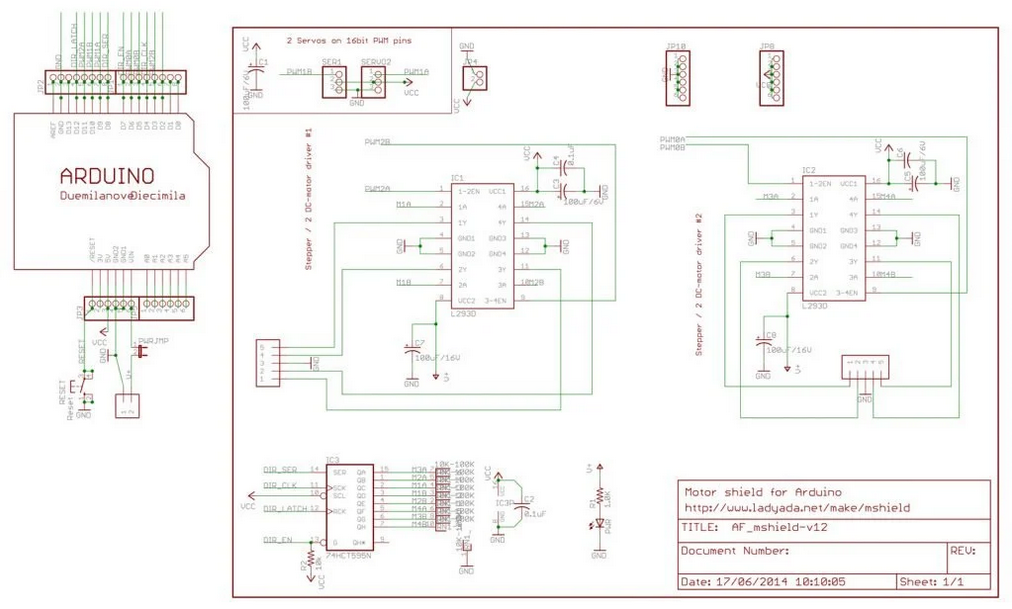
\includegraphics[scale=.3]{Media/Figuren/Motorshield_SCHEM.png}
%     \caption{Motorshield schematische tekening}
%     \label{MSCHEM}
% \end{figure}


% Met behulp van de timingtabel in figuur \ref{Timing} heb ik code geschreven waarmee we de 8-bits code uit figuur \ref{MCode} kunnen sturen naar het motorshield.
% \begin{figure}[h]
%     \centering
%     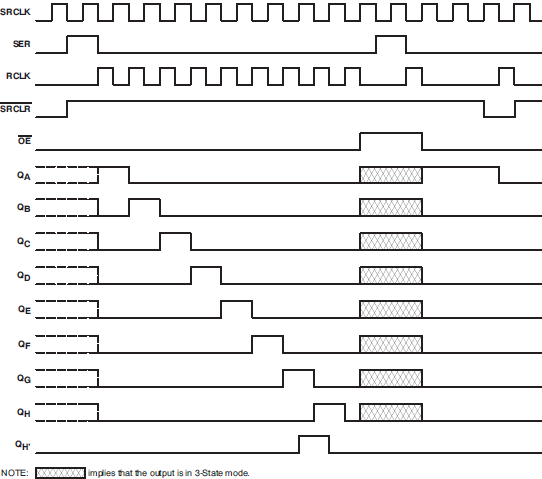
\includegraphics[scale=.5]{Media/Figuren/Timing.PNG}
%     \caption{Motorshield timing}
%     \label{Timing}
% \end{figure}

% \begin{figure}[h]
%     \begin{lstlisting}
%     void MOTOR(int Direction, int MotorPWM1, int MotorPWM2, int MotorPWM3, int MotorPWM4) {
%   SPEED(MotorPWM1, MotorPWM2, MotorPWM3, MotorPWM4);
%   digitalWrite(DIR_LATCH, LOW);
%   shiftOut(DATA, DIR_CLK, MSBFIRST, Direction);
%   digitalWrite(DIR_LATCH, HIGH);}
%     \end{lstlisting}
%     \caption{Motorshield code}
%     \label{MCode}
% \end{figure}

% Met behulp van deze informatie heb ik een Excel-script geschreven waarmee we konden aangeven welke motor moest draaien en in welke richting. Deze gegevens hebben we later naar het shiftregister gestuurd, dat de H-brug aanstuurt.